\chapter{はじめに}
\section{モチベーション}
日常生活の中で私たち人間は,容易に
人間の「印象」を得ることができる.
例えば,
「落ち着いた人」や「信頼できそうな人」といったものである.
また,そういった印象は主に顔から与えられるものである.

ここで,同じようにコンピュータが人の顔を入力として受け取った時,
人の印象を出力するシステムを構築することは可能だろうか?
人工知能が人間の印象を識別することは可能だろうか?

また,人の印象というのは必ずしも一つに限定されない.
「落ち着いていて,信頼できそうな人」といったように,
人間の印象は複数得られうる.

そこで,私は,
「{\bf 男性の顔写真を入力として,その顔の「印象」を複数出力する
システムの作成}」を実験テーマとした,

このようなタスクを機械学習に行わせることを{\bf マルチラベル問題}
という.サンプルに対する正解が1つに限定されるマルチクラス問題と
比較して,マルチラベル問題にはさまざまな技術的な困難が伴う.
また,マルチラベル問題は不均衡なデータ(imbalanced data)を
扱うことになりやすく,その点でも困難が伴う.
このような技術的な課題に挑戦することもこのテーマを選択した
動機である.
\section{全体像}
今回私は,「{\bf 男性の顔写真を入力として,その顔の「印象」を複数出力する
システム}」を作成する.システムのイメージを図
\ref{fig:ch1:system}
に示す.

\begin{figure}[tb]
  \centering
  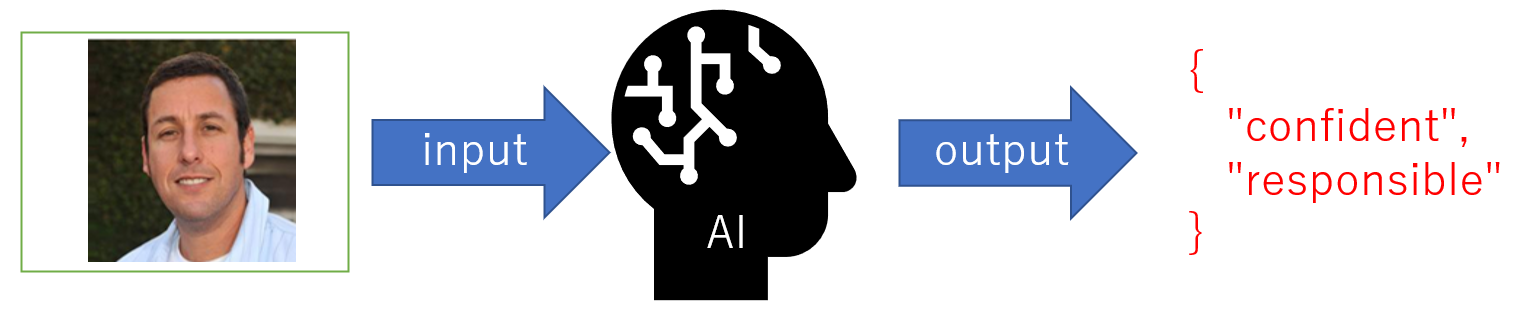
\includegraphics[width=13cm]{ch1/system.png}
  \caption{
  システムの全体像のイメージ
  \label{fig:ch1:system}
  }
\end{figure}

男性の顔写真を機械学習システムに入力すると,
事前に設定された7の印象のうち,
顔写真がどの印象に該当するかを複数出力する.

顔写真を男性に限定する理由は,
人間の印象は性別により判断基準が大きく異なると予想され,
実験の予算内で収集できる少ないデータでは,
すべての性別に対応する機械学習システムを作成することは難しいと
考えられたためである.

システムに設定される7つの印象を以下にに示す.

\begin{quote}
  {\small
  caring, confident, 
  emotionally stable, intelligent, 
  responsible, sociable,
  trustworthy }
\end{quote}
  
これは海外の認知科学系の研究で主に使われている
13の顔の印象(impression)\cite{doi:10.1073/pnas.1807222115}のうち,
主にネガティブな意味を含む印象を削除したものである.

印象の数が多いと機械学習がうまくいかないリスクが高まる.
また,近年ではクラウドソーシングを用いたデータの
ラベリングが,倫理的な問題を引き起こしかねないことが
知られている\cite{ai-rinri}.

今回のテーマでは
実在する人間の顔写真に,クラウドソージングで印象のラベリングを行う.
そのため,ネガティブな印象を削除することは
倫理的な問題を回避するためにもよい選択であると考えられる.
\\

このレポートでは,中間発表までの取り組みを実験1,
最終発表までの取り組みを実験2として説明する.
つづく第2章では実験1の内容を,クラウドソージング・前処理・機械学習の順に説明し,
第3章では同様に実験2を説明する.
実験1・2では,クラウドソージングによってデータを調達し,
適切な手法を用いて機械学習を行い,
テストデータでその性能を評価することで,
システムを作成・評価する.最終章の第4章では,結果の考察と今後の課題について議論する.